\chapter{Dokumentacja}

\section{Diagramy klas}

\begin{center}
	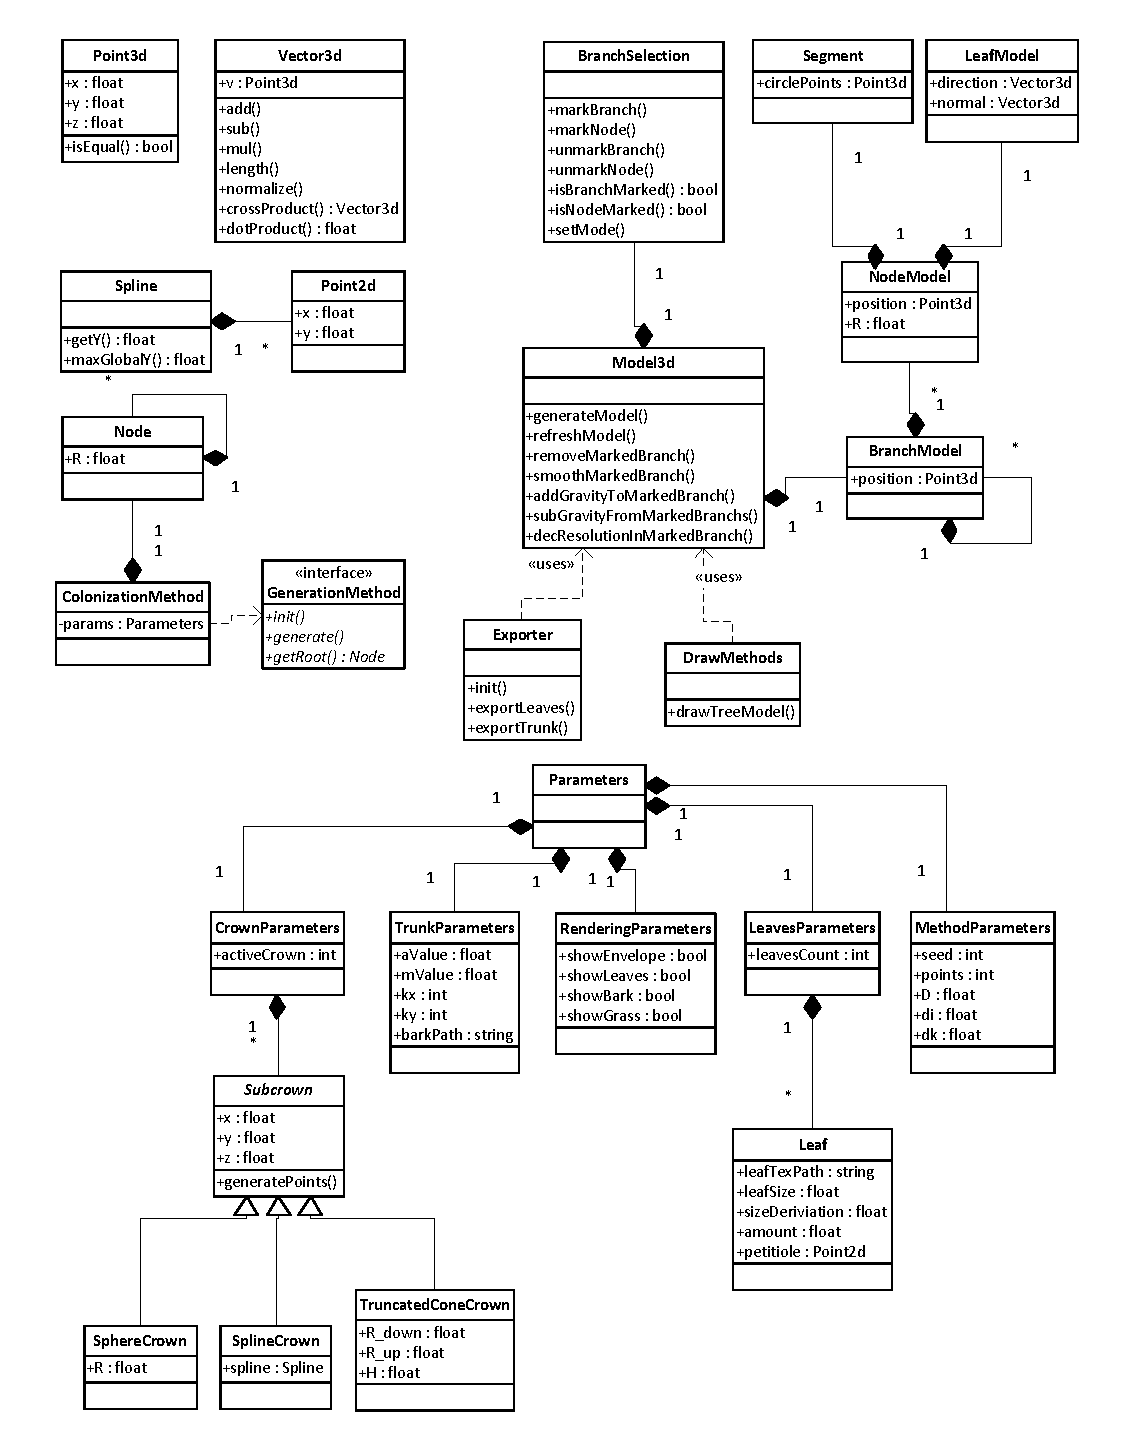
\includegraphics[scale=0.55]{images/treemaker_uml}
	\label{treemaker_uml}
\end{center}

\section{Eksport modelu}
Ponieważ format danych używany w programie nie jest zgodny z powszechnie uznanymi formatami modeli trójwymiarowych, aby zachować kompatybilność należy przeprowadzić eksport modelu do 
formatu zewnętrznego. Format .OBJ zgodnie z wymaganiami jest obsługiwany przez program Blender.
Został on opracowany przez firmę Wavefront Technologies i ze względu na swoją prostotę stał się szybko
popularny wśród programów do obróbki grafiki trójwymiarowej. Na format składa się plik tekstowy z rozszerzeniem .obj 
zawierający opis geometrii obiektu. Dodatkowo format przewiduje odwołanie do pliku z rozszerzeniem .mtl zawierającym
opis materiałów (kolorów i tekstur).


\subsection{Struktura pliku .obj}
Plik jest podzielony na linie, z czego każda linia moze zawierać:
\begin{itemize}
\item '\#' : komentarz 
\item mtllib [nazwa pliku .mtl] :odwołanie do pliku z materiałami
\item usemtl [nazwa materiału]  :nakaz użycia materiału
\item o [nazwa obiektu]         :definicję obiektu
\item g [nazwa grupy]           :definicję grupy: 
\item v [x] [y] [z]             :współrzędne wierzchołka
\item vn [x] [y] [z]            :współrzędne wektora normalnego
\item vt [x] [y]                :współrzędne tekstury
\item f [v1/vn1/vt1] [v2/vn2/vt2] [v3/vn3/vt3] :definicja trójkąta 
\end{itemize}
Warto nadmienić, iż przy definiowaniu trójkątów podajemy indeksy (numerowane od 1) poszczególnych współrzędnych znajdujących się w pliku.
Istotne jest również to, iż współrzędne tekstury i wektora normalnego trójkąta są opcjonalne. Sam wektor normalny może być odtworzony poprawnie,
nawet jeśli nie został zawarty w pliku, dzięki podaniu współrzędnych wierzchołków zgodnie z ruchem wskazówek zegara.


\subsection{Struktura pliku .mtl}
Plik .mtl może zawierać definicje wielu materiałów. Podobnie jak plik .obj jest to plik tekstowy z informacjami znajdującymi
się w kolejnych liniach mogących zawierać:
\begin{itemize}
\item '\#' : komentarz 
\item newmtl [nazwa materiału]: definicja materiału
\item Ka [r] [g] [b]: \textit{ambient color}
\item Kd [r] [g] [b]: \textit{diffuse color}
\item Ks [r] [g] [b]: \textit{specular color}
\item Ns [x]        : \textit{specular cooef}
\item d  [x]        : przeźroczystość
\item map\_Ka [nazwa pliku]: tekstura 
\end{itemize}


\subsection{Procedura eksportu}
Model drzewa jest eksportowany w dwóch etapach, jako dwie osobne grupy jednego obiektu. Pierwszą grupę stanowi pień drzewa, natomiast drugą jego liście.
Pozwala to na użycie różnych tekstur dla tych elementów drzewa. Program grupuje współrzędne wierzchołków i tekstur by zmniejszyć rozmiar tworzonego pliku, a następnie
zapisuje je do pliku \{models/tree0.obj\}. Dodatkowo program tworzy plik \{models/tree0.mtl\} zawierający opis materiałów i ścieżek do tekstur. 
\section{Opis interfejsu użytkownika}

\subsection{Okno główne}
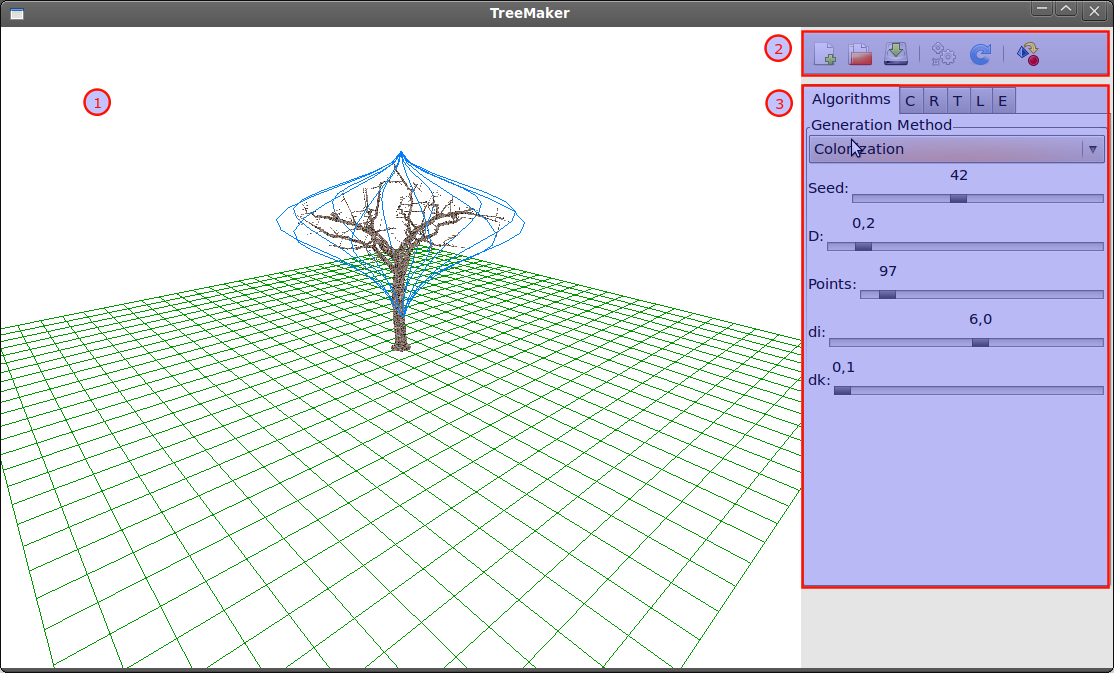
\includegraphics[width=120mm]{images/gui/main_window.png}
\begin{enumerate}
	\item {Podgląd wygenerowanego modelu drzewa.}
	\item {Przybornik.}
	\item {Panel z ustawieniami generatora.}
\end{enumerate}

\subsection{Podgląd wygenerowanego modelu}
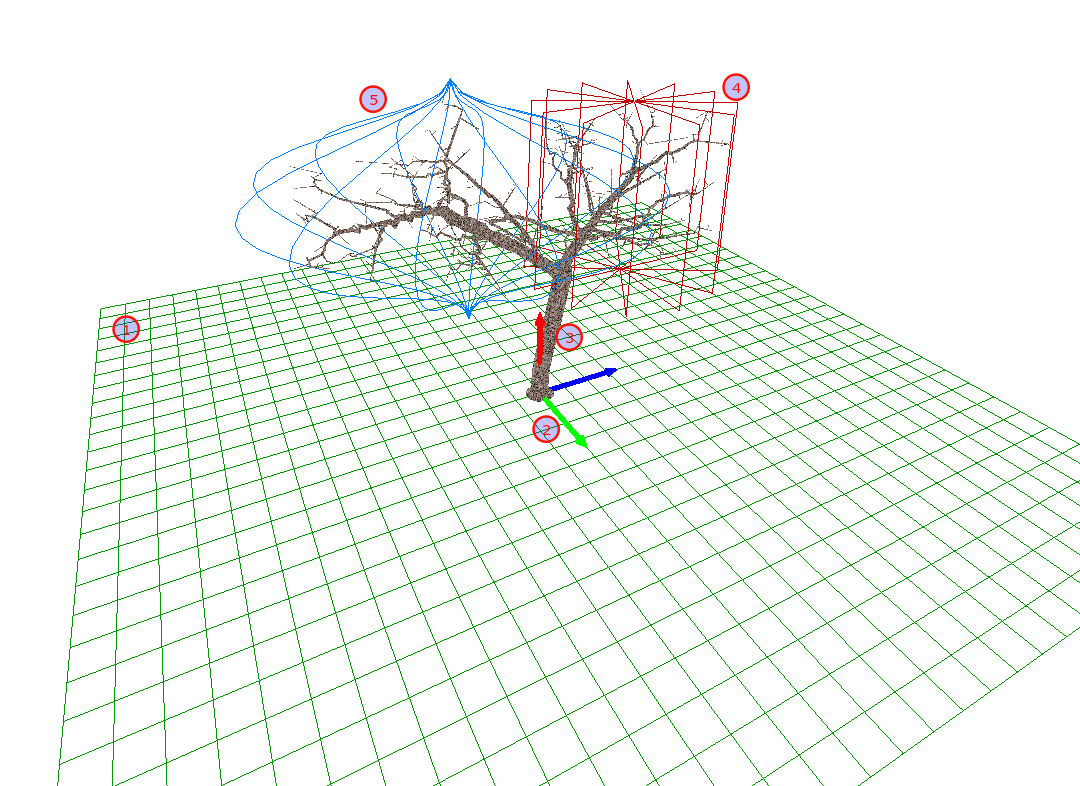
\includegraphics[width=120mm]{images/gui/model_view.png}
\begin{enumerate}
	\item {Siatka wyznaczająca poziom ziemi.}
	\item {Układ współrzędnych.}
	\item {Model drzewa.}
	\item {Aktywna korona.}
	\item {Nieaktywna korona.}
\end{enumerate}

\subsection{Przybornik}
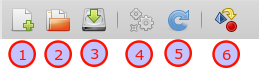
\includegraphics[width=50mm]{images/gui/toolbar.png}
\begin{enumerate}
	\item {Resetuj konfigurację - ustawia domyślne wartości wszystkich parametrów.}
	\item {Wczytaj konfigurację - wczytuje konfigurację programu z pliku. }
	\item {Zapisz konfigurację - zapisuje konfigurację do pliku.}
	\item {Generuj nowy model - tworzy nowy model na podstawie parametrów widocznych w zakładce \textit{Algorithms}, \textit{C}(ustawienia koron), \textit{T}(ustawienia dotyczące modelowania pnia), \textit{L}(ustawienia liści).}
	\item {Odśwież model - model jest uaktualniany korzystając z parametrów zawartych w zakładce \textit{L} oraz \textit{T}. Nie jest wywoływany algorytm generowania drzewa.}
	\item {Eksportuj model - model drzewa jest eksportowany do formatu OBJ. Tworzone są dwa pliki \textit{models/tree0.obj} oraz \textit{models/tree0.mtl}.}
\end{enumerate}

\subsection{Opcje algorytmu}
\begin{threeparttable}
\begin{tabular}{lr}
\parbox[c]{95mm}{
\begin{enumerate}
	\item {Wybór algorytmu generującego drzewo.}
	\item {Ziarno generatora pseudo-losowego.}
	\item {Odległość pomiędzy sąsiednimi węzłami w drzewie.}
	\item {Liczba atraktorów, z których generowane jest drzewo.}
	\item {Influence distance - odległość w jakiej węzły drzewa poszukują atraktorów.}
	\item {Kill distance - odległość od atraktora do węzła drzewa po osiągnięciu której atraktor jest usuwany.}
\end{enumerate}
} &
\parbox[c]{35mm}{
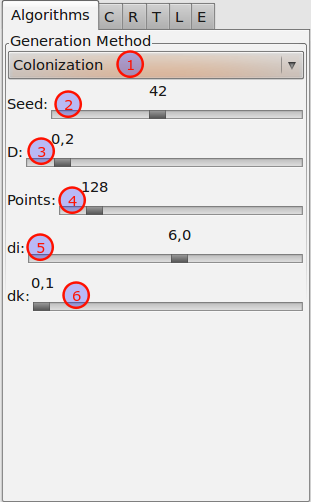
\includegraphics[width=35mm]{images/gui/algorithms_panel.png}
}\\
\end{tabular}
\end{threeparttable}


\subsection{Opcje korony}
\begin{threeparttable}
\begin{tabular}{lr}
\parbox[c]{95mm}{
\begin{enumerate}
	\item {Typ korony - do wyboru: sfera, ścięty stożek, \textit{spline crown}.}
	\item {Dodaj koronę - dodaje koronę do generatora.}	
	\item {Lista dodanych koron - koron może być więcej niż 1. Atraktory są rozmieszczane we wszystkich koronach z listy(w każdej jest identyczna liczba atraktorów równa $liczba\_atraktorów/liczba\_koron$).}
	\item {Współrzędna X wybranej korony.}
	\item {Współrzędna Y wybranej korony.}
	\item {Współrzędna Z wybranej korony.}
	\item {Usuń wybraną koronę.}
	\item {Parametry charakterystyczne dla każdego typu korony.}
\end{enumerate}
} &
\parbox[c]{35mm}{
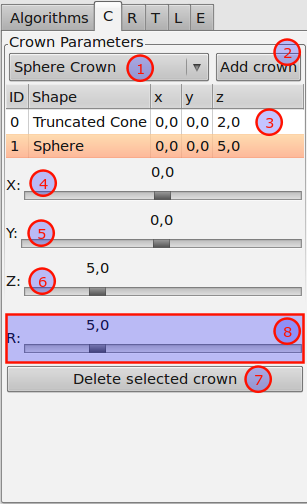
\includegraphics[width=35mm]{images/gui/crown_panel.png}
}\\
\end{tabular}
\end{threeparttable}

\subsubsection{Sfera}
\begin{threeparttable}
\begin{tabular}{lr}
\parbox[c]{95mm}{
\begin{enumerate}
	\item {Promień sfery.}
\end{enumerate}
} &
\parbox[c]{35mm}{

\includegraphics[width=35mm]{images/gui/sphere_crown.png}
}\\
\end{tabular}
\end{threeparttable}

\subsubsection{Ścięty stożek}
\begin{threeparttable}
\begin{tabular}{lr}
\parbox[c]{95mm}{
\begin{enumerate}
	\item {Wysokość.}
	\item {Promień górnej podstawy.}
	\item {Promień dolnej podstawy.}
\end{enumerate}
} &
\parbox[c]{35mm}{
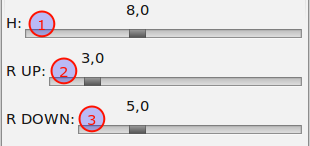
\includegraphics[width=35mm]{images/gui/truncated_cone_crown.png}
}\\
\end{tabular}
\end{threeparttable}

\subsubsection{\textit{Spline crown}}
\begin{threeparttable}
\begin{tabular}{lr}
\parbox[c]{95mm}{
\begin{enumerate}
	\item {Lista z węzłami interpolującymi.}
	\item {Dodaj węzeł interpolujący.}
	\item {Usuń węzeł interpolujący.}
	\item {Współrzędna X wybranego węzła interpolującego.}
	\item {Współrzędna Y wybranego węzła interpolującego.}
\end{enumerate}
} &
\parbox[c]{35mm}{
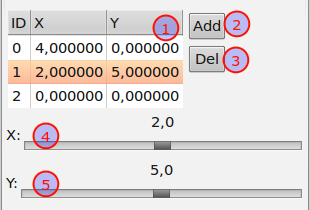
\includegraphics[width=35mm]{images/gui/spline_crown.png}
}\\
\end{tabular}
\end{threeparttable}

\subsection{Opcje wyświetlania}
\begin{threeparttable}
\begin{tabular}{lr}
\parbox[c]{95mm}{
\begin{enumerate}
	\item {Wyświetla dodane korony.}
	\item {Wyświetla liście.}
	\item {Wyświetla korę.}
	\item {Wyświetla trawę.}
\end{enumerate}
} &
\parbox[c]{35mm}{
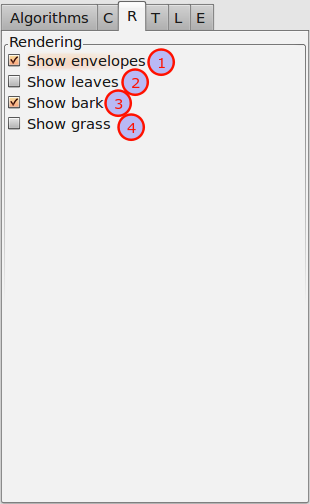
\includegraphics[width=35mm]{images/gui/rendering_panel.png}
}\\
\end{tabular}
\end{threeparttable}


\subsection{Opcje pnia}
\begin{threeparttable}
\begin{tabular}{lr}
\parbox[c]{95mm}{
\begin{enumerate}
	\item {Współczynnik $radius factor$. Wpływa na grubość pnia przy łączeniu gałęzi. $\tnote{1}$}
	\item {Współczynnik $a$.$\tnote{1}$}
	\item {Współczynnik $m$.$\tnote{1}$}
	\item {Liczba punktów tworzących segment.}
	\item {Liczba tekstur potrzebną do owinięcia pnia.}
	\item {Stosunek rozmiaru tekstury do odległości mierzonej wzdłuż pnia.}
\end{enumerate}
} &
\parbox[c]{35mm}{
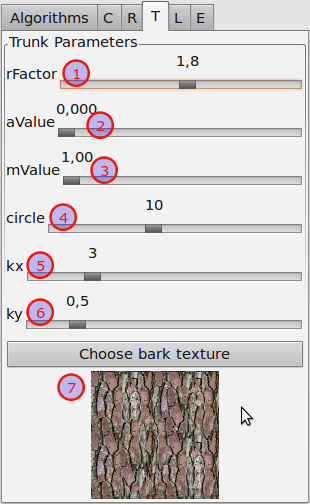
\includegraphics[width=35mm]{images/gui/trunk_panel.png}
}\\
\end{tabular}
\begin{tablenotes}
	\item[1] Wpływ współczynników na wygląd pnia dokładnie opisany w podrozdziale \ref{subsec:node_model} na stronie \pageref{subsec:node_model}.
\end{tablenotes}

\end{threeparttable}

\subsection{Opcje liści}
\begin{threeparttable}
\begin{tabular}{lr}
\parbox[c]{95mm}{
\begin{enumerate}
	\item {Liczba liści doczepianych do wygenerowanego modelu.}
	\item {Lista rodzajów liści.}
	\item {Rozmiar danego liścia.}
	\item {Maksymalne odchylenie wielkości liści.}
	\item {Współczynnik wpływający na liczbę liści danego typu.}
	\item {Dodawanie nowego typu liścia.}
\end{enumerate}
} &
\parbox[c]{35mm}{
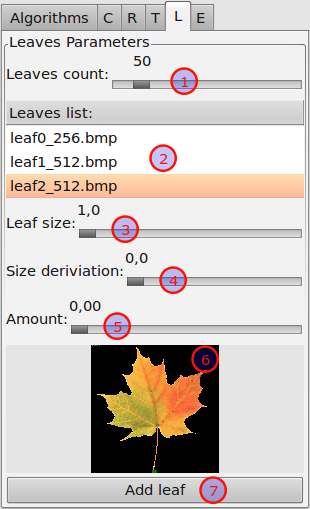
\includegraphics[width=35mm]{images/gui/leaves_panel.png}
}\\
\end{tabular}
\end{threeparttable}



\subsection{Edytor}
\begin{threeparttable}
\begin{tabular}{lr}
\parbox[c]{95mm}{
\begin{enumerate}
	\item {Tryb zaznaczania gałęzi - odpowiednio: cała gałęź, od punktu do końca gałęzi oraz od punktu do punktu.}
	\item {Zastosuj dla wszystkich dzieci - edycji podlegają też gałęzie wychodzące z edytowanego fragmentu i dalej rekursywnie wszyscy potomkowie.}
	\item {Przycinanie gałęzi.}
	\item {Wygładzanie gałęzi - gałęzie są modyfikowane przy użyciu algorytmu Chaikina.}
	\item {Zmniejszanie rozdzielczości gałęzi - co drugi węzeł gałęzi jest usuwany. Gałęzie wychodzące z usuwanych węzłów są przesuwane do węzłów położonych niżej.}
	\item {Dociążanie gałęzi - od współrzędnej $Z$ danego węzła jest odejmowana pewna stała, która rośnie wprost proporcjonalnie do odległości węzła od osi drzewa.}
	\item {Odciązanie gałęzi - analogicznie do opcji 6.}
\end{enumerate}
} &
\parbox[c]{35mm}{
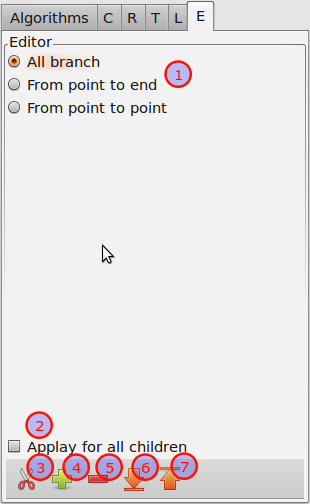
\includegraphics[width=35mm]{images/gui/editor_panel.png}
}\\
\end{tabular}
\end{threeparttable}

\section{Kompilacja projektu}
\subsection{Wymagane biblioteki}
Zgodnie z wymaganiami programi powinien posiadać możliwie małą ilość zależności. System powinien posiadać kompilator GCC oraz bibliotekę GTK+ z rozszerzeniem do obsługi OpenGL.
Poniżej przedstawiono dokładne wersje bibliotek wymagane przez program.
\begin{itemize}
\item GTK+ 2.2
\item GTKGLEXT 1.2
\item MESA 7.8
\item GCC 4.4.4
\end{itemize}
\subsection{Uruchomienie}
Źródła programu zostały załączone na płycie CD, ponadto znajdują się na stronie https://code.google.com/p/treemaker/source/browse/.\\
Po ich pobraniu wystarczy wydać polecenie make w katalogu ze źródłami by rozpocząć kompilację programu. Jeśli przebiegła ona pomyślnie został utworzony
program wykonywalny o nazwie treemaker.
